\section{Experiments}
\label{sec:experiments}

We organize the evidence into four questions: the accuracy and
finite-horizon reliability of local specialists  prediction, the benefit of
cross-regime routing and fusion, the behavior of internal routing
and physical-field diagnostics, and the computational cost.
The three benchmarks provide complementary : flow pass a Circular case supplies controlled local comparisons, flow pass a Square  case supplies the principal history-conditioned fusion study, and Fluidic Pinball case
provides an archived POD--Galerkin comparison and additional overlap
results. Their configurations and horizons are summarized in
Table~\ref{tab:chart_splits}.



\subsection{Local prediction accuracy and finite-horizon reliability}
\label{sec:exp_local}

\paragraph{Comparison with POD--Galerkin.}
Table~\ref{tab:pinball_autonomous}  
 comparison  local specialists with classical POD--Galerkin over
$K=32$--$56$ steps. Table~\ref{tab:pinball_autonomous} show local specialists achieves low physical-field errors across all four evaluation settings. Compared with POD--Galerkin, the learned specialists consistently reduce both velocity and pressure errors, with the largest differences appearing in pressure. For example, the Hopf joint error decreases from $48.94\%$ to $2.085\%$, while the standard Periodic error decreases from $43.20\%$ to $0.8415\%$. The longer-horizon Periodic-core evaluation shows the same trend, with $E_{\mathrm{joint}}$ reduced from $41.91\%$ to $1.672\%$. Together, these results show that the learned specialists maintain low physical-field error over the evaluated autonomous horizons. In particular, compared with POD-Garlerkin, by incorporating a sparse mixture-of-experts correction into the projected Galerkin equation, the local specialists substantially reduce the
long-horizon error.


\begin{table}[H]
\centering
\caption{
Autonomous local-specialist prediction on the fluidic-pinball benchmark. Errors are physical-field percentages; lower is better. Periodic-core denotes the longer-horizon periodic evaluation; complete protocol details are given in Appendix~\ref{app:pinball}.
}
\label{tab:pinball_autonomous}
\small
\setlength{\tabcolsep}{5pt}
\begin{tabular}{@{}llrrr@{}}
\toprule
Evaluation setting & Model & $E_u$ & $E_p$ & $E_{\mathrm{joint}}$ \\
\midrule
Steady ($K=56$)
& POD--Galerkin
& -- & -- & -- \\
& RAL-MoE-ROM
& 0.2247 & 0.7593 & 0.9840 \\
\addlinespace

Hopf ($K=56$)
& POD--Galerkin
& 0.4378 & 48.50 & 48.94 \\
& RAL-MoE-ROM
& 0.0995 & 1.986 & 2.085 \\
\addlinespace

Periodic ($K=32$)
& POD--Galerkin
& 1.641 & 41.56 & 43.20 \\
& RAL-MoE-ROM
& 0.2897 & 0.5518 & 0.8415 \\
\addlinespace

Periodic-core ($K=56$)
& POD--Galerkin
& 2.555 & 39.36 & 41.91 \\
& RAL-MoE-ROM
& 0.6222 & 1.050 & 1.672 \\
\bottomrule
\end{tabular}
\end{table}

\paragraph{Controlled local comparisons.}
We compare Circular Hopf and Periodic predictors on common held-out
windows at $K=24$ and $K=48$, using seeds 1248, 1600, and 2026 for
the neural configurations. Dense matches the proposed model's active
neural parameter budget, while Structured retains explicit response
branches but removes input-dependent expert routing. These are
controls for the local architecture, not substitutes for a bare
POD--Galerkin ablation. We also include a validation-selected
operator inference (OpInf) fit as an external ROM comparison.
The repaired configurations change the initialization of the
low-rank quadratic factors; they are retrained models, not a
post-hoc modification of the original predictions.

Table~\ref{tab:circular_full_reorg} brings together both regimes and
horizons under the same full-window joint-error metric.
Reference fields are reconstructed from true POD coefficients, so
these errors exclude the original CFD projection remainder.
Evaluation windows, aggregation, component errors, and implementation
details are provided in Appendix~\ref{app:circular}.

\begin{table}[t]
\centering
\small
\setlength{\tabcolsep}{4pt}
\caption{Circular local controls: full-window joint error
$E_u+E_p$ (\%) against POD-reconstructed reference fields.
Neural entries are mean $\pm$ sample standard deviation over accepted
seeds among three attempts. Accepted seed sets can differ between
configurations; 2/3 rows are conditional descriptive statistics,
not complete three-seed estimates. Repaired Hopf rows use FP32.
OpInf is a single deterministic validation-selected fit.
The two horizons use the same windows, with $K=24$ restricted to
their first 24 steps.}
\label{tab:circular_full_reorg}
\begin{tabular}{@{}llccc@{}}
\toprule
Regime & Model & $K=24$ & $K=48$ & Accepted\\
\midrule
Hopf & Proposed, original
& $0.11521\pm0.08694$ & $0.11487\pm0.10033$ & 2/3\\
& Proposed, repaired
& $0.04334\pm0.02379$ & $0.05044\pm0.03439$ & 2/3\\
& Dense, active-matched
& $0.15406\pm0.16364$ & $0.15480\pm0.15525$ & 2/3\\
& Structured, original
& $0.12537\pm0.04614$ & $0.12724\pm0.04302$ & 3/3\\
& Structured, repaired
& $0.02229\pm0.00432$ & $0.02392\pm0.00778$ & 2/3\\
& OpInf & 0.03870 & 0.05340 & Deterministic\\
\midrule
Periodic & Proposed, original
& $2.8791\pm1.7269$ & $4.9443\pm3.1576$ & 3/3\\
& Proposed, repaired
& $3.0667\pm1.8373$ & $5.5322\pm3.6623$ & 3/3\\
& Dense, active-matched
& $\mathbf{1.3251\pm0.2268}$ & $\mathbf{2.3998\pm0.6599}$ & 3/3\\
& Structured, original
& $2.8666\pm1.4342$ & $5.2810\pm2.5679$ & 3/3\\
& Structured, repaired
& $2.8598\pm1.3081$ & $5.0677\pm2.3762$ & 3/3\\
& OpInf & 114.0941 & 114.9897 & Deterministic\\
\bottomrule
\end{tabular}
\end{table}

\paragraph{Accuracy under matched local controls.}
All Periodic neural configurations have three accepted seeds.
Dense yields lower mean joint errors than the proposed configurations
at both horizons, while Structured is close to the original proposed
model. Under this active-parameter budget and evaluation protocol,
the results therefore do not establish a Periodic accuracy advantage
from input-dependent sparse routing. Errors increase when extending
the window from 24 to 48 steps; neither low finite-window error nor
successful completion proves arbitrary-time stability.

\paragraph{Initialization and training reliability.}
The original Circular quadratic branches remain inactive because
both multiplicative factors were initialized at zero.
Retaining one random factor while zeroing the other permits learning,
but the repaired Proposed model does not improve the Periodic mean
error. Retraining also changes optimization and checkpoint selection,
so this comparison does not isolate the quadratic term alone.
For Hopf, repaired FP32 configurations have only two accepted seeds
per architecture, and their accepted sets differ from the original
ones. Their lower conditional errors consequently do not establish
improved expected performance or complete three-seed robustness.
Appendix~\ref{app:circular} reports the initialization mechanism and
Table~\ref{tab:hopf_completion} distinguishes training failure from
validation rejection.

\paragraph{Comparison with operator inference.}
OpInf is competitive on Hopf at both horizons but substantially less
accurate on Periodic in this task-specific fit.
Its Periodic regularization choice lies at the upper boundary of the
searched grid, limiting interpretation of the poor result.
Together with the different pressure parameterization and derivative
estimation described in Appendix~\ref{app:circular}, this prevents
a general claim of superiority over the OpInf method family.

\subsection{Cross-regime routing and physical-space fusion}
\label{sec:exp_fusion}

We hold the Square local predictors and E2 router fixed and compare
assembly rules on the prescribed S--H and H--P support at $K=24$.
Each interface contains 16 held-out windows.
E2 Top-1 selects within the supplied pair; T2-C learns a correction
to its pair preference using initial-history descriptors.
Neither the candidate set nor an automatic applicability mask is
learned in this experiment.

Table~\ref{tab:routing_fusion} uses a common full-window metric.
Train-fixed $\alpha$ and train-fixed logit offset are fitted only
on training windows, and the fixed candidate is selected on
validation error. These controls test whether the improvement
can be explained by a constant mixture or calibration offset.

\begin{table}[H]
\centering
\small
\caption{Square full-window joint error (\%) at $K=24$ against the
cached POD reference. Entries use the frozen-checkpoint reevaluation,
not a three-seed average. Scalar controls use training data;
the fixed candidate uses validation data.}
\label{tab:routing_fusion}
\begin{tabular}{@{}lrr@{}}
\toprule
Assembly rule & S--H & H--P\\
\midrule
E2 Top-1 & 1.5786 & 1.6424\\
E2-probability blend & 1.8145 & 1.4489\\
Equal blend & 2.3849 & 1.3930\\
Train-fixed $\alpha$ & 2.0591 & 0.9767\\
Train-fixed logit offset & 2.0149 & 0.9821\\
Validation-fixed candidate & 1.5786 & 1.0068\\
T2-C & \textbf{1.0954} & \textbf{0.8123}\\
\bottomrule
\end{tabular}
\end{table}

T2-C improves on all listed controls for these fixed candidate
sets. A separate architecture-matched $\mu$-only control zeros the
standardized history channels while retaining the gate architecture.
Across three paired gate seeds, full-window joint errors are
$1.095351\pm0.000015\%$ versus $1.814699\pm0.000242\%$
in S--H and $0.812343\pm0.000177\%$ versus
$0.976939\pm0.000179\%$ in H--P.
The reductions are $39.64\%$ and $16.85\%$.
These quantify gate-training variability, not uncertainty from
retraining the complete hierarchy.

\begin{figure}[H]
\centering
% Source: audited three-gate-seed full-window means; no field pixels generated.
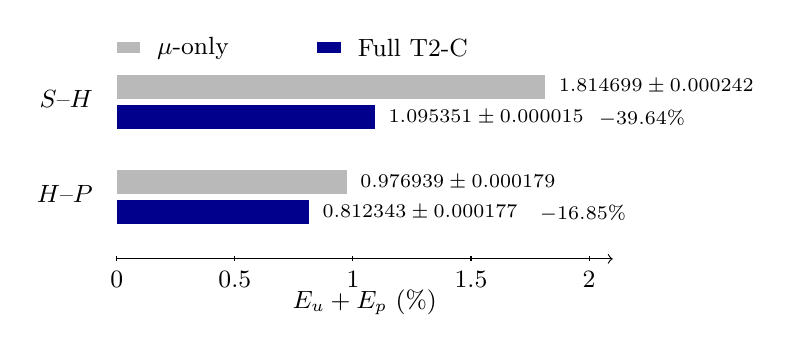
\begin{tikzpicture}[x=3cm,y=0.55cm,font=\small]
\draw[->] (0,0)--(2.1,0);
\node at (1.05,-1.0) {$E_u+E_p$ (\%)};
\foreach \t in {0,0.5,1,1.5,2} {
 \draw (\t,0.06)--(\t,-0.06) node[below] {\t};
}
\node[anchor=east] at (-0.06,3.7) {$S$--$H$};
\node[anchor=east] at (-0.06,1.5) {$H$--$P$};
\fill[gray!55] (0,3.7) rectangle (1.814699,4.25);
\fill[blue!55!black] (0,3.0) rectangle (1.095351,3.55);
\fill[gray!55] (0,1.5) rectangle (0.976939,2.05);
\fill[blue!55!black] (0,0.8) rectangle (0.812343,1.35);
\node[anchor=west,font=\scriptsize] at (1.83,3.975) {$1.814699\pm0.000242$};
\node[anchor=west,font=\scriptsize] at (1.11,3.275) {$1.095351\pm0.000015$};
\node[anchor=west,font=\scriptsize] at (0.99,1.775) {$0.976939\pm0.000179$};
\node[anchor=west,font=\scriptsize] at (0.83,1.075) {$0.812343\pm0.000177$};
\fill[gray!55] (0,4.75) rectangle (0.1,5.0);
\node[anchor=west] at (0.13,4.87) {$\mu$-only};
\fill[blue!55!black] (0.85,4.75) rectangle (0.95,5.0);
\node[anchor=west] at (0.98,4.87) {Full T2-C};
\node[anchor=west,font=\scriptsize] at (2.0,3.25) {$-39.64\%$};
\node[anchor=west,font=\scriptsize] at (1.75,1.05) {$-16.85\%$};
\end{tikzpicture}

\caption{Full-window Square comparison over three paired gate seeds.
All local candidates and E2 are fixed; bars show mean and sample
standard deviation.}
\label{fig:square_overlap}
\end{figure}

The evidence supports history-conditioned fusion for these windows,
but does not prove that history dependence is necessary for every
flow or gate. The weight is fixed within each prediction window;
history can change it between windows.
Appendix~\ref{app:square} retains component errors, terminal-step
results, scalar objectives, and complete field visualizations.
Additional Pinball overlap results appear in
Appendix~\ref{app:pinball_overlap_results}; their local candidates
are Deep-FNN-H3, so they test the assembly interface rather than
the sparse-MoE architecture.
A posteriori convex oracles are diagnostics, not deployable methods.

\subsection{Internal routing and physical-field diagnostics}
\label{sec:exp_diagnostics}

\paragraph{Expert utilization.}
Post-hoc diagnostics use frozen Circular H/P specialists and are
not used for checkpoint selection.
Periodic distributes decisions across group--pair combinations;
Hopf has a prescribed single group and fixed sparse support, but
nonuniform, parameter-dependent mixture weights.
Its single group is not evidence of collapse of a learned
multi-group router. The detailed frequency, weight-mass, and entropy
statistics in Appendix~\ref{app:internal_routing} count the first
integration stage per output step, not all RK evaluations.
Utilization alone does not establish an accuracy benefit.

\paragraph{Fusion consistency.}
Appendix~\ref{app:fusion_consistency} separates conditional algebraic
identities from measured reconstructed-field diagnostics.
On both Square interfaces, the measured T2-C pressure residual is
lower than either candidate for both tested spatial stencils.
However, Hopf has a smaller H--P momentum residual and a smaller
S--H energy error. Fusion is therefore not a general residual or
energy-error minimizer.

The measurements use offline least-squares spatial derivatives
and coarse-time differences, not the original OpenFOAM
finite-volume residuals. Nonzero reference residuals include POD
truncation and differentiation error.
Identity discrepancies near machine precision verify the algebra,
not conservation or physical accuracy.
The phase screen resolves none of the 16 S--H windows and 15 of
16 H--P windows; even resolved short-window traces do not establish
absence of aliasing or long-time phase stability.
The complete energy, residual, probe, and phase curves are retained
in Appendix~\ref{app:fusion_measured}.

\subsection{Computational cost and timing boundaries}
\label{sec:exp_cost}

Sparse activation is a parameter-use property, not a runtime claim.
Circular H/P activate $44.53\%$ and $17.09\%$ of their trainable
parameters per analyzed prediction decision.
For native Circular Periodic prediction at batch size one and
$K=48$, median times are 2.1848 s (proposed), 0.6579 s (Dense),
and 0.8652 s (Structured).
The proposed implementation is therefore slower than Dense in this
measurement despite sparse activation; the native Galerkin path
also executes on the CPU.

A separate warm physical-input/physical-output measurement includes
history encoding, local advancement, and all-step field decoding.
It takes 2.18747 s on an RTX 4090 with a Xeon host for a Circular
Periodic window spanning 598.70093 physical time units.
A matched historical production FOM interval takes 1996 s.
The resulting ratio of approximately 912.5 is not a full-hierarchy
or hardware-independent speedup: hardware and I/O boundaries differ,
the FOM timing has one realization, and ROM loading, output writes,
E2, descriptors, and T2-C are excluded.
Appendix~\ref{app:parameter_counts} lists warm-ups, repetitions,
synchronization, memory, hardware, and all included/excluded work.
A fully paired Top-2 end-to-end timing remains unmeasured.
